\def\version{1}
\problemname{Labyrinth Construction}
Let us define a \textit{labyrinth} as follows:
\begin{enumerate}
  \item The labyrinth consists of $K$ rooms, where some pairs of rooms are connected by corridors.
  \item It is possible to get between every pair of rooms by walking through a sequence of corridors.
  \item No room has a corridor to itself.
  \item There may be several corridors connecting the same pair of rooms.
  \item Every corridor has one of three colors: red, green or blue.
  \item Every room has exactly three corridors, one of each color.
  \item One room is the entrance of the labyrinth, and one room is the exit of the labyrinth (these are different rooms).
\end{enumerate}

The sisters Rosa and Lila are playing a game where Rosa first constructs a labyrinth, after which Lila tries to complete it by walking from the entrance to the exit.
They have played a few times now, and Lila always manages to win.
This makes Rosa rather frustrated.
She wants her sister to be stuck in the labyrinth forever.

Rosa has noticed, however, that Lila always uses the same predictable strategy.
More precisely, she has a string $S$ consisting of the letters \texttt{R}, \texttt{G} and \texttt{B} (red, green and blue), whose length we write as $|S|$.
On move number $t$, Lila looks at the $t$th character and follows the corridor of the color that the letter represents (so if the letter is \texttt{R}, Lila will walk through the red corridor of the room she is currently in).
After $|S|$ moves she starts over by looking at the first character again.
In other words, if the string is \texttt{RGB} she will first walk through the red corridor of the entrance, then the green corridor of the room she arrived in, then the blue corridor, then the red one (she has now started reading the string from the beginning again), green, blue, red, and so on.
Note that every room has exactly one corridor of each color, so the room she goes to at each step is uniquely determined.

\begin{figure}[h!]
  \centering
  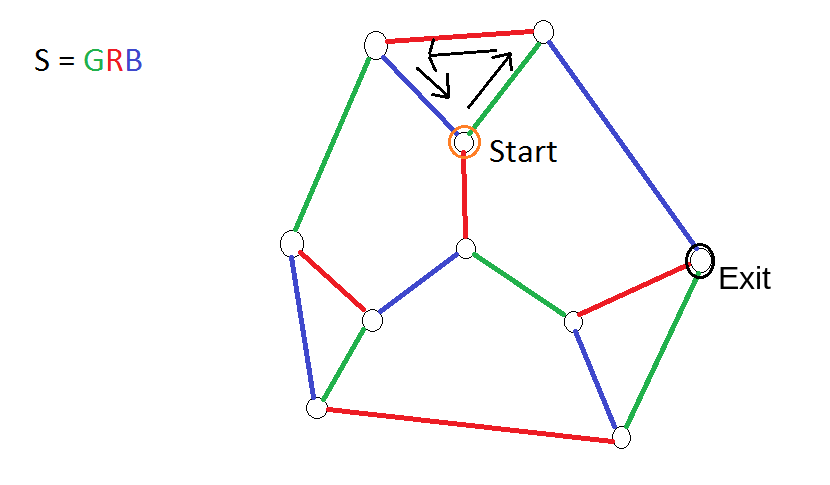
\includegraphics[width=0.6\textwidth]{labyrintgraf2.en.png}
  \caption{An example labyrinth.}
\end{figure}

Given $S$, your task is to construct a labyrinth that Lila can never complete.

\section*{Input}
The input contains the string $S$ ($3 \leq |S| \leq 400\,001$), consisting of the letters \texttt{R}, \texttt{G} and \texttt{B}.

In this problem you can additionally download all of the input at the bottom of the page.

\section*{Output}
Begin by printing three integers $K$, $i$ and $u$ ($2 \leq K \leq 2|S|$, $0 \leq i,u < K$, $i \neq u$).
$K$ should be the number of rooms in the labyrinth you construct.
$i$ and $u$ should be the zero-indexed numbers (that is, between $0$ and $K - 1$) of the rooms that are the entrance and the exit of the labyrinth.

Then print $K$ lines, one for each room, ordered by room number starting with room $0$.
The line for room $j$ should contain three integers $r$, $g$ and $b$ ($0 \leq r,g,b < K$) -- the rooms that the red, green and blue corridors of room $j$ lead to, respectively.

Your labyrinth must satisfy the conditions in the problem description.

\section*{Scoring}
In total the problem has $11$ test cases, one of which is the sample.
You are not scored on the sample, but on the $10$ remaining test cases.

Let $K_{\min}$ be the number of rooms in the smallest labyrinth that any contestant managed to construct for a given test case during the contest, and let $K$ be the number of rooms in your labyrinth.
Let
$$r_1 = \frac{K}{K_{\min}}$$
and
$$r_2 = \frac{2|S|}{K_{\min}}$$
where $|S|$ is the length of the string $S$.

Your score on that test case is then
$$\min\left(10, 10 \cdot \left(1 - \frac{\log(r_1)}{\log(r_2)}\right)\right),$$
or $0$ if $K$ exceeds $2|S|$.
